\documentclass{article}

\usepackage{graphicx}
\usepackage{tikz}
\usepackage{tikzsymbols}
\usetikzlibrary{calc,patterns,shapes.geometric}
\pagestyle{empty}
\usepackage[margin=0pt]{geometry}
\geometry{papersize={14in,12in}}

\def\centerarc[#1](#2)(#3:#4:#5){\draw[#1] ($(#2)+({#5*cos(#3)},{#5*sin(#3)})$) arc (#3:#4:#5);}

\begin{document}
	\begin{figure}
		\centering
		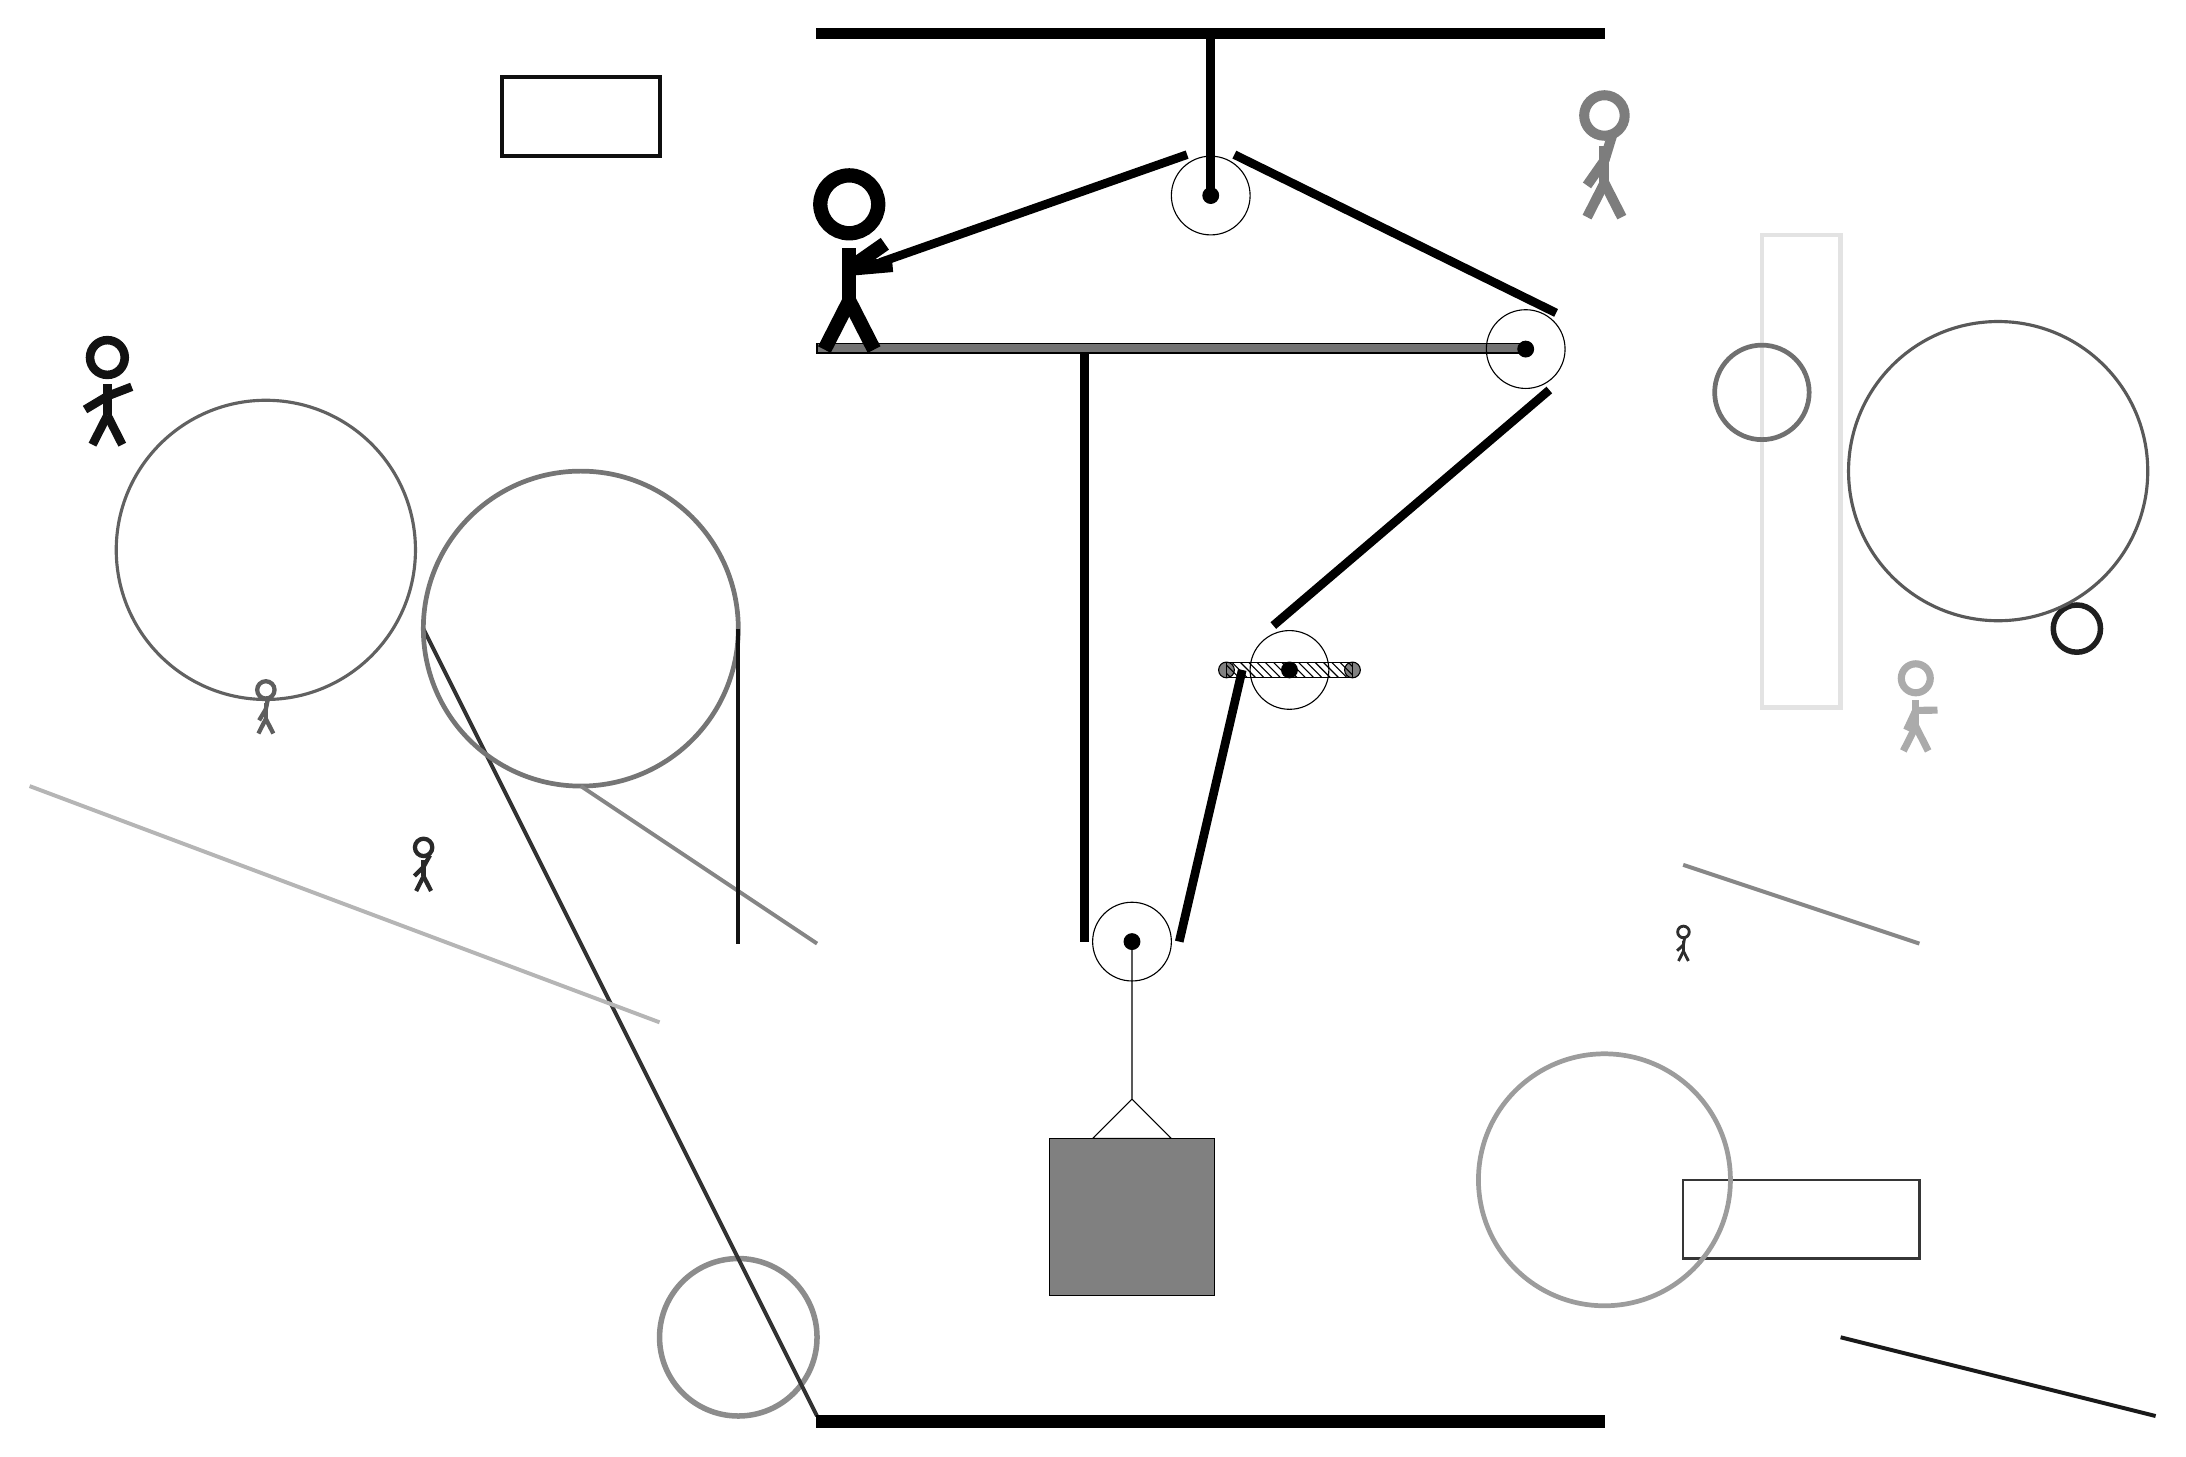
\begin{tikzpicture}
			%%%%% START %%%%%
			
			\draw[fill=black] (-2, 15.5) rectangle (8, 15.625);
			
			\draw[fill=black!55] (-2, 11.5) rectangle (7, 11.625);
			
			\draw (2, 4.025) circle (0.5);
			\draw[fill=black] (2, 4.025) circle (0.1);
			
			\draw (7, 11.55) circle (0.5);
			\draw[fill=black] (7, 11.55) circle (0.1);
			
			\draw[fill=white](4, 7.475) circle (0.5);
			\draw[fill=black] (4, 7.475) circle (0.1);
			\draw[fill=black!50] (3.2, 7.475) circle (0.1);
			\draw[fill=black!50] (4.8, 7.475) circle (0.1);
			\draw[pattern=north west lines, pattern color=black] (3.2, 7.575) rectangle (4.8, 7.375);
			
			\draw (3, 13.5) circle (0.5);
			\draw[fill=black] (3, 13.5) circle (0.1);
			\draw[line width=1.1mm] (3, 13.5) -- (3, 15.5);
			
			\draw (2, 4.025) -- (2, 2.025) -- (1.5, 1.525) -- (2.5, 1.525) -- (2, 2.025);
			\draw[fill=black!50] (0.95, 1.525) rectangle (3.05, -0.475);
			
			\draw[line width=1.1mm] (1.4, 11.5) -- (1.4, 4.025);
			\centerarc[line width=1.1mm](2, 4.025)(180:360:0.6);
			\draw[line width=1.1mm](2.6, 4.025) -- (3.4, 7.475);
			\centerarc[line width=1.1mm](4, 7.475)(110:180:0.6);
			\draw[line width=1.1mm](3.7948, 8.0388) -- (7.3, 11.0304);
			\centerarc[line width=1.1mm](7, 11.55)(-60:50:0.6);
			\draw[line width=1.1mm](7.3857, 12.0096) -- (3.3, 14.0196);
			\centerarc[line width=1.1mm](3, 13.5)(60:120:0.6);
			\draw[line width=1.1mm](2.7, 14.0196) -- (-1.2, 12.65);
			
			\draw[line width=0.5mm, color=black!90](11, -1) -- (15, -2);
			
			\draw [line width=0.7mm, color=black!45](-3, -1) circle (1.0);
			\node[line width=0.7mm, color=black!51] at (8, 14) {\Strichmaxerl[7][55][73]};
			\draw[line width=0.3mm, color=black!79] (9, 1) rectangle (12, 0);
			
			\draw[line width=0.5mm, color=black!80](-7, 8) -- (-2, -2);
			\draw[line width=0.5mm, color=black!94] (-4, 14) rectangle (-6, 15);
			
			\node[line width=0.5mm, color=black!82] at (9, 4) {\Strichmaxerl[2][43][81]};
			\draw [line width=0.6mm, color=black!54](-5, 8) circle (2.0);
			\draw [line width=0.4mm, color=black!62](-9, 9) circle (1.9);
			\draw [line width=0.6mm, color=black!39](8, 1) circle (1.6);
			\draw[line width=0.5mm, color=black!48](-2, 4) -- (-5, 6);
			\node[line width=0.5mm, color=black!93] at (-11, 11) {\Strichmaxerl[6][31][21]};
			\node[line width=0.7mm, color=black!63] at (-9, 7) {\Strichmaxerl[3][59][79]};
			
			\draw[line width=0.6mm, color=black!11] (10, 7) rectangle (11, 13);
			\draw[line width=0.5mm, color=black!93](-3, 8) -- (-3, 4);
			\draw [line width=0.7mm, color=black!88](14, 8) circle (0.3);
			\node[line width=0.6mm, color=black!84] at (-7, 5) {\Strichmaxerl[3][45][61]};
			\node[line width=0.2mm, color=black!33] at (12, 7) {\Strichmaxerl[5][65][1]};
			\draw [line width=0.4mm, color=black!65](13, 10) circle (1.9);
			\draw[line width=0.5mm, color=black!29](-4, 3) -- (-12, 6);
			\draw [line width=0.6mm, color=black!56](10, 11) circle (0.6);
			
			\draw[line width=0.5mm, color=black!47](12, 4) -- (9, 5);
			
			
			\node at (-1.5, 12.65) {\Strichmaxerl[10][-175][35]};
			
			\draw[fill=black] (-2, -2) rectangle (8, -2.15);
			
			%%%%% END %%%%%
		\end{tikzpicture}
	\end{figure}	
\end{document}